\chapter{相关背景知识}

\section{混沌工程与故障注入}

故障注入是一类主动验证系统可靠性的方法。它通过人为制造错误、延迟、资源耗尽或数据异常，观察系统是否能够维持预期行为。早期故障注入常用于硬件、操作系统和分布式系统测试，后来在云原生环境中发展为混沌工程。Basiri 等将混沌工程定义为在分布式系统上进行实验，以建立系统面对生产环境中动荡条件时仍能承受的信心\cite{basiri2016chaos}。该思想强调先定义稳态假设，再受控引入故障，并通过观测数据判断系统是否偏离稳态。

Netflix 的 Chaos Monkey 是混沌工程的代表性实践。它通过随机终止生产环境中的虚拟机实例，迫使系统具备单点失效容忍能力\cite{netflixChaosMonkey}。其后，Chaos Toolkit、LitmusChaos、Chaos Mesh 等工具进一步扩展了实验描述、执行和回滚能力。Chaos Toolkit 使用 JSON/YAML 描述稳态假设、探针和动作，使实验语义与底层实现相对解耦\cite{chaosToolkit}。Chaos Mesh 则面向 Kubernetes 环境，通过 CRD 注入网络、Pod、IO、时间和 JVM 等故障。

这些工具的共同特点是面向资源层或平台层。它们擅长回答“某个 Pod 被杀掉后系统是否恢复”“网络延迟上升后服务是否超时”“CPU 被压满后请求延迟如何变化”等问题。但在 AI 原生应用中，一些关键故障发生在应用内部：某个工具返回合法但错误的数据，某个状态 reducer 接收空值，某个 LangGraph 条件边被错误选择，某个 LLM 结构化输出缺字段。这些故障不一定伴随容器崩溃或网络故障，却会直接影响智能体决策和用户结果。因此，本文关注的应用层故障注入并不是替代资源层混沌工程，而是在更贴近智能体语义的位置补充故障模型。

\section{Agent 评估与 AgentOps}

Agent 评估通常关注任务完成率、工具调用正确性、多轮一致性、幻觉率、成本和延迟等维度。与传统模型评测相比，Agent 评估更难，因为一次输出往往由多个模型调用、工具调用和状态更新共同决定。一个失败结果可能来自提示词不充分，也可能来自检索数据缺失、工具异常、状态覆盖或下游服务失败。

AgentOps 平台试图通过 Trace、会话、数据集、评估器和人工标注来解决这一问题。LangSmith 为 LangChain/LangGraph 应用提供运行记录、Trace 可视化、数据集评测和 Prompt 迭代能力\cite{langsmithDocs}。AgentOps 等平台也提供对 LangGraph 工作流的节点执行、工具使用、状态变化和耗时信息的追踪\cite{agentopsLangGraph}。这些工具的价值在于让开发者“看见”Agent 行为，从而定位错误和优化提示词或工具。

图~\ref{fig:agentops-comparison} 展示了传统系统运维与智能体系统运维的关注点差异。传统运维主要围绕服务、资源和接口状态展开，而 AgentOps 需要进一步观测模型调用、工具执行、规划轨迹、记忆状态和多轮会话过程\cite{wang2025surveyagentopscategorizationchallenges}。这说明 AI 原生应用的可靠性问题不再只存在于基础设施和服务边界，也存在于智能体运行时的语义链路中。

\begin{figure}[htbp]
  \centering
  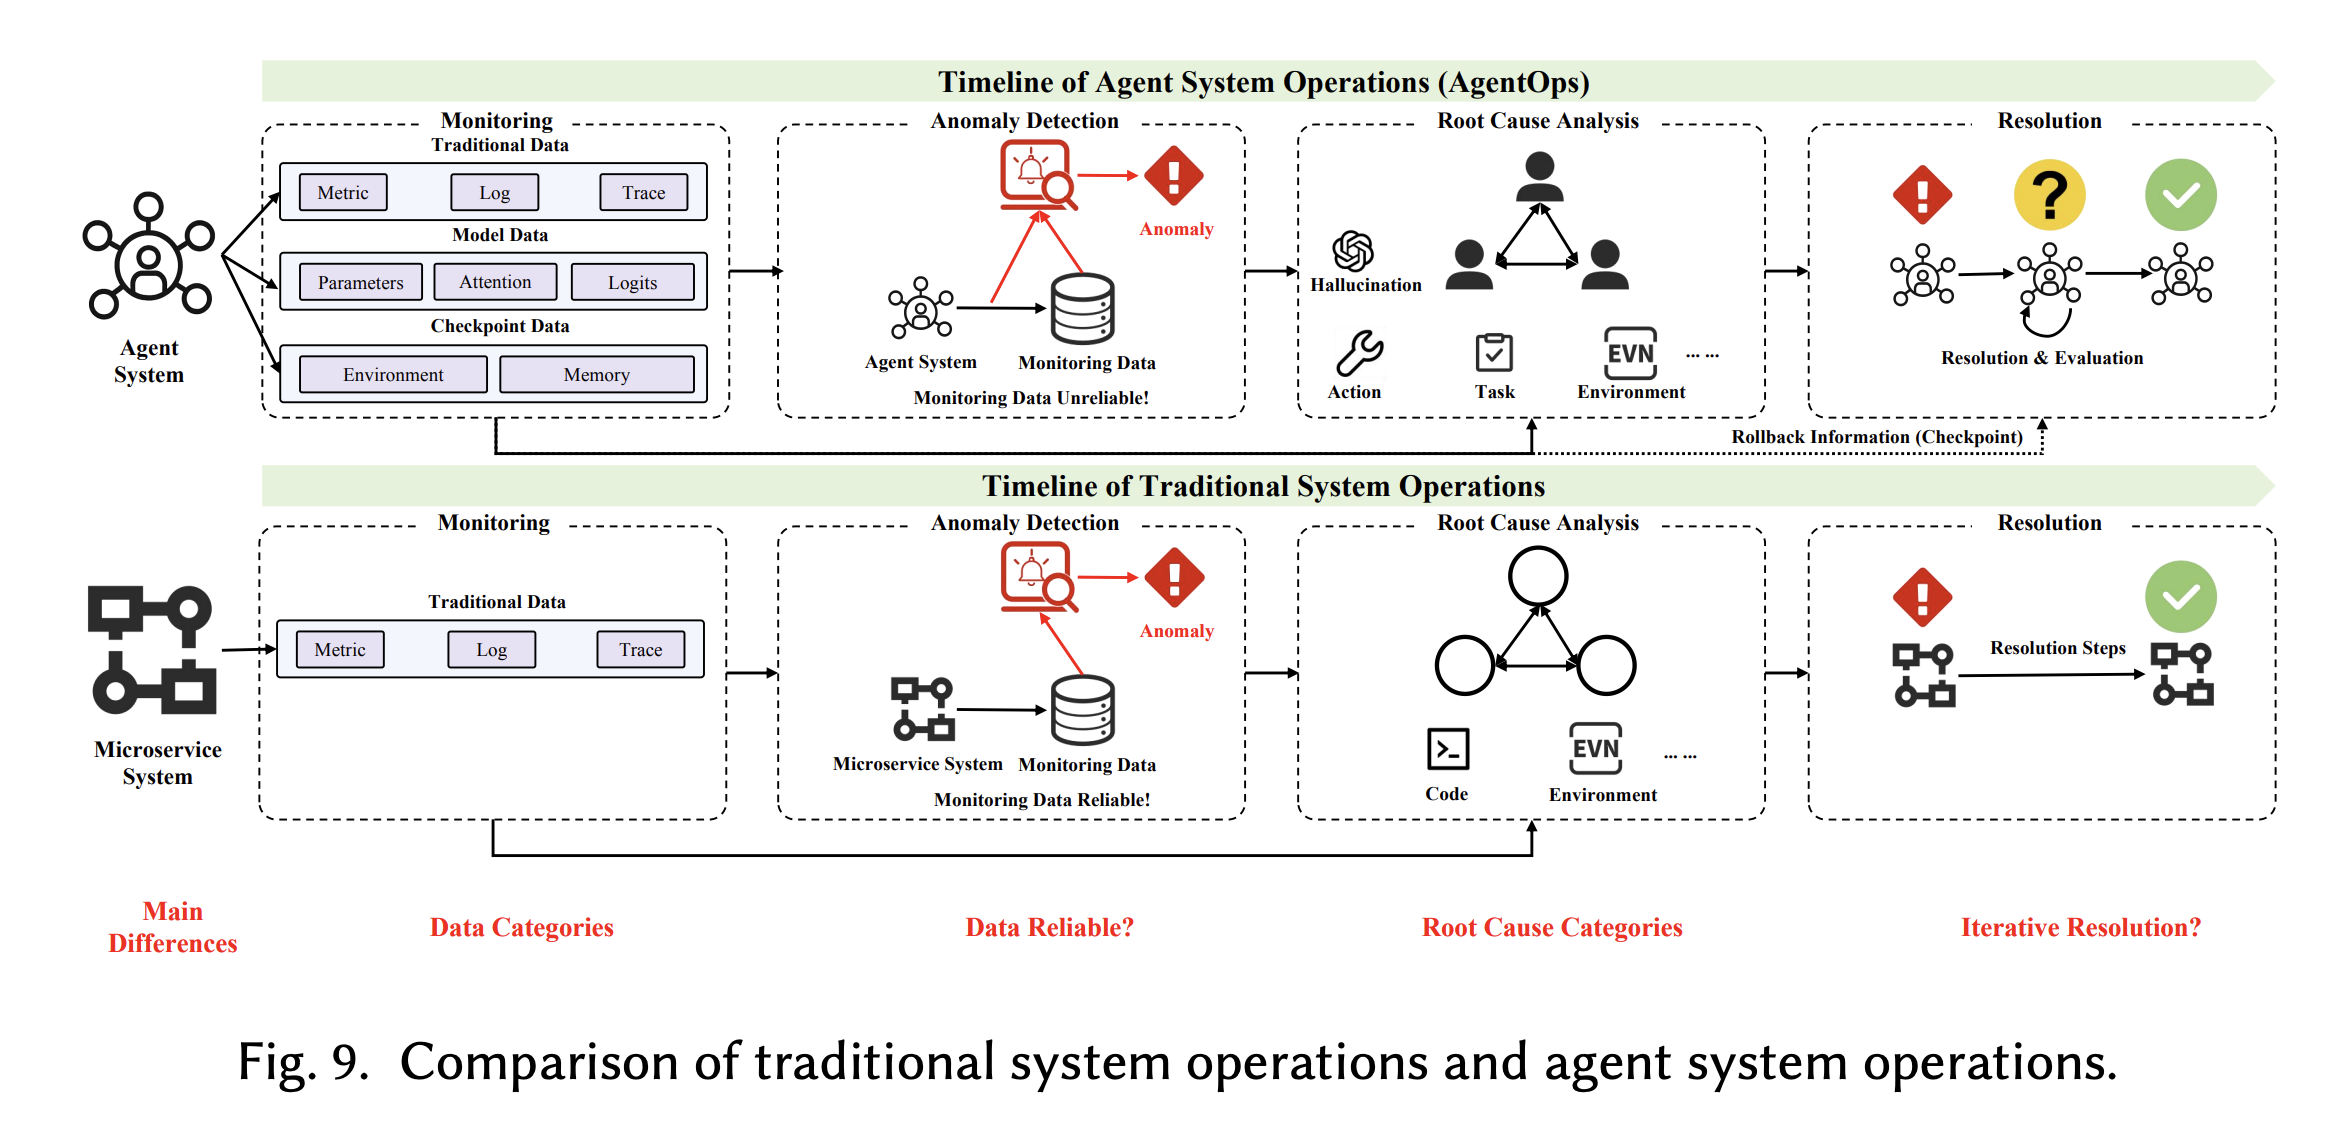
\includegraphics[width=\textwidth]{figures/Comparison of traditional system operations and agent system operations.png}
  \caption{传统系统运维与智能体系统运维对比\cite{wang2025surveyagentopscategorizationchallenges}}
  \label{fig:agentops-comparison}
\end{figure}

然而，AgentOps 平台通常以观测和评估为主，缺少稳定制造系统坏境的能力。现实中的 Bad Case 往往难以复现：同一个问题下次调用模型可能生成不同答案，某个第三方 API 的短时故障难以再次出现，某个状态同步错误只在特定多轮上下文中发生。本文将故障注入放在 AgentOps 之前或旁边：先通过可控注入制造故障，再用 Trace 和评估工具分析系统反应。这样可以把一次偶发 Bad Case 转化为可复跑实验。

\section{OpenTelemetry 与 GenAI 可观测}

OpenTelemetry 已成为分布式系统可观测性的事实标准之一。它通过 Trace、Metric 和 Log 三类信号描述系统行为，并使用 Span 表示一次操作在调用树中的位置、耗时、属性和事件。对于传统微服务，HTTP、数据库和 RPC 的语义约定已经较成熟；对于 AI 原生应用，社区正在推进 GenAI 相关语义约定。

OpenTelemetry GenAI 语义约定提出了模型调用、Agent 调用、工具执行和生成式 AI 指标的标准字段。例如，Agent 调用可以使用 \code{gen\_ai.operation.name=invoke\_agent}，工具执行可以使用 \code{execute\_tool}，模型相关指标可以记录 \code{gen\_ai.client.operation.duration}、\code{gen\_ai.server.time\_to\_first\_token} 等\cite{otelGenAIAgentSpans,otelGenAIMetrics}。OpenTelemetry 官方博客也指出，随着 LangGraph、CrewAI、AutoGen 等智能体框架进入生产环境，统一的智能体语义约定对跨平台可观测和可靠性分析变得重要\cite{otelAgentObservability}。

这些标准化工作为本文提供了两个启发。第一，AI 原生应用的观测对象正在从“单个 LLM 请求”扩展为“Agent 图、工具节点、状态变化和会话级执行”。第二，故障注入证据也应落在这些观测对象上。本文在 TripSphere 中使用 \code{experiment.id}、\code{fault.scenario}、\code{fault.injected}、\code{fault.target}、\code{fault.primitive}、\code{fault.outcome} 等属性，使故障事件可以与 Span 绑定。这样既符合 OpenTelemetry 的可观测范式，也为未来迁移到更标准的 GenAI 语义字段留下空间。

\section{LangGraph 状态图}

LangGraph 是 LangChain 生态中面向有状态智能体和工作流的编排框架。它将执行过程表示为图：节点可以是 LLM 调用、工具执行或普通函数；边可以是固定边，也可以是根据状态动态选择的条件边；状态由类型化结构承载，并在节点之间传递和更新\cite{langgraphDocs}。这种模型适合表达多步规划、ReAct 循环、人机协作和持久化会话。

以 LangGraph 官方 RAG Agent 示例为例，图~\ref{fig:langgraph-rag-agent} 中的检索、答案生成、查询改写和结果评估节点通过条件边连接，构成一个可循环的状态图\cite{langgraphAgenticRag}。这种结构使智能体可以根据中间状态动态选择下一步动作，但也意味着错误状态、空检索结果或路由扰动可能沿图传播。

\begin{figure}[htbp]
  \centering
  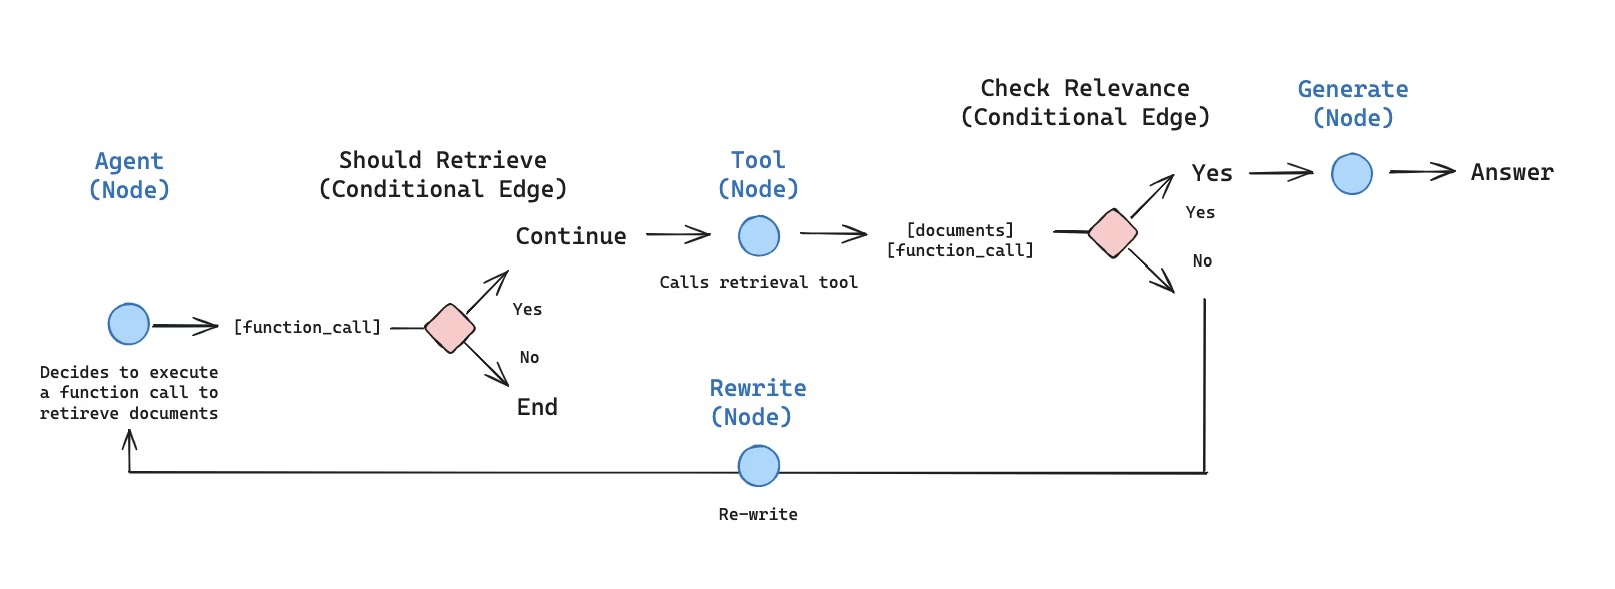
\includegraphics[width=0.86\textwidth]{figures/Build a custom RAG agent with LangGraph.png}
  \caption{LangGraph 自定义 RAG Agent 状态图示例\cite{langgraphAgenticRag}}
  \label{fig:langgraph-rag-agent}
\end{figure}

LangGraph 的优势也带来了新的可靠性问题。状态更新可能被错误覆盖，条件路由可能进入错误分支，工具节点可能返回部分成功结果，checkpointer 的持久化策略会影响恢复行为。对于简单脚本，这些问题可能只表现为一次异常；对于 AI 原生应用，它们会在多轮对话和跨服务调用中传播，最终影响用户看到的行程、订单或推荐。因此，LangGraph 的节点、边、状态和工具边界不仅是业务实现单元，也是应用层故障注入和观测证据采集的重要位置。

\section{本文定位}

综合来看，现有研究和工具分别覆盖了三个方向：混沌工程提供资源层主动实验能力，AgentOps 提供智能体行为观测和评估能力，OpenTelemetry GenAI 语义约定提供跨平台可观测标准。本文的定位是在三者之间补齐“面向 AI 原生应用层的可复现故障注入”。

与传统混沌工程相比，本文更关注单条请求、单个工具、单段状态和单次 Agent turn 的精确注入。与 AgentOps 相比，本文更强调主动制造故障和实验复现，而不是单纯记录运行结果。与通用可观测标准相比，本文提供了面向 TripSphere 和 LangGraph 的具体工程落地，并把故障声明、命中证据和实验指标纳入同一条证据链。下一章将不再抽象讨论 AI 原生应用框架，而是结合 TripSphere 的真实组件，将其拆解为用户交互、Agent 编排、工具与外部服务、业务微服务以及可观测与实验控制五个层次，并在这些层次之间确定故障注入边界。
